\documentclass[openany]{book}

\usepackage{paralist}
\usepackage{rotating}
\usepackage{listings}

\usepackage[usenames,dvipsnames,svgnames,table]{xcolor}
\usepackage{tabularx}
\usepackage[utf8]{inputenc}
\usepackage[ngerman]{babel}
\usepackage{geometry}
\geometry{
	left = 1cm,
	right = 1cm,
	top = 2cm,
	bottom = 2cm
}

%\usepackage{showframe}% http://ctan.org/pkg/showframe
\usepackage{titlesec}
%\titleformat{\chapter}[hang] 
%{\normalfont\huge\bfseries}{\chaptertitlename\ \thechapter:}{1em}{} 

\titleformat{\chapter}[hang] 
{\normalfont\huge\bfseries}{\chaptertitlename\ \thechapter:}{1em}{}

%\titleformat{\chapter}[display]
%{\normalfont\huge\bfseries}{\chaptertitlename\ \thechapter:}{1em}{}

% this alters "before" spacing (the second length argument) to 0
\titlespacing*{\chapter}{0pt}{0pt}{10pt}
\titlespacing*{\section}{5pt}{0pt}{5pt}

\usepackage{amssymb} 
\usepackage{amsmath}
\usepackage{mathtools}
\usepackage[autostyle]{csquotes}
\usepackage{graphicx}


\usepackage[colorlinks]{hyperref}
\hypersetup{
	colorlinks = false,
	linkbordercolor= red
}

\usepackage{algorithm}
\usepackage[noend]{algpseudocode}
\usepackage{listings}
\lstset{	
	commentstyle=\it,
	emphstyle={\bf\ttfamily},
	stringstyle=\mdseries\ttfamily,	
	keywordstyle=\bfseries\ttfamily,
	basicstyle=\small\ttfamily,	
	numberstyle=\ttfamily\tiny\color[gray]{0.3},
	tabsize=4,	
	%xleftmargin=2pt,
	%stepnumber=1,
	%numbers=left,
	%numbersep=5pt,
	%  belowcaptionskip=\bigskipamount,
	%  captionpos=b,
	%  escapeinside={*'}{'*},
	%  showspaces=false,
	%showstringspaces=false,
	%morecomment=[l]\%,
	%escapeinside={<@}{@>},
}


\setlength{\marginparwidth}{2cm}
\usepackage[colorinlistoftodos,prependcaption,textsize=small]{todonotes}
\newcommand{\unsure}[2][]{\todo[linecolor=red,backgroundcolor=red!25,bordercolor=red,#1]{#2}}
\newcommand{\change}[2][]{\todo[linecolor=blue,backgroundcolor=blue!25,bordercolor=blue,#1]{#2}}
\newcommand{\info}[2][]{\todo[linecolor=OliveGreen,backgroundcolor=OliveGreen!25,bordercolor=OliveGreen,#1]{#2}}
\newcommand{\improvement}[2][]{\todo[linecolor=Plum,backgroundcolor=Plum!25,bordercolor=Plum,#1]{#2}}
\newcommand{\notdone}[1]{\todo[linecolor=Fuchsia,backgroundcolor=Fuchsia!25,bordercolor=Fuchsia,inline]{Noch nicht geschrieben: #1}}
\newcommand{\skipped}{\todo[linecolor=Fuchsia,backgroundcolor=Fuchsia!25,bordercolor=Fuchsia,inline]{Ausgelassen.}}
\newcommand{\thiswillnotshow}[2][]{\todo[disable,#1]{#2}}
\newcommand{\open}{\colorbox{red}{Todo}}

\setcounter{secnumdepth}{3}
\setcounter{tocdepth}{3}

\renewcommand\thepart{\arabic{part}}
\newcommand{\myparagraph}[1]{\paragraph{#1}\mbox{}\\}
\newcommand{\funcSignature}[1]{\paragraph{$#1$}\mbox{}\\}
\newcommand{\example}{\newline Bsp.:}
\newcommand{\explain}{\newline Erklärung: \newline}
\newcommand{\constraint}{\newline \newline Constraint: \newline \newline}
\newcommand{\equal}{\newline Äquivalent: \newline}
\newcommand{\analog}[1]{\newline \underline{Analog:} $#1$ \newline}
\newcommand{\slide}[2]{(Folie: $#1\_\text{(#2)}$)}
\newcommand{\engquote}[1]{\foreignblockquote{english}{#1}}
\newcommand{\multlineTable}[1]{\begin{tabular}[c]{@{}l@{}}\\#1\\ \end{tabular}}
\definecolor{light-gray}{gray}{0.9}
\newcommand{\exRef}[1]{ \colorbox{light-gray}{(Ref.: #1)}}




\DeclarePairedDelimiter\ceil{\lceil}{\rceil}
\DeclarePairedDelimiter\floor{\lfloor}{\rfloor}

\begin{document}

%\begin{algorithm}
%	\caption{template $a+b=c$}
%	\begin{algorithmic}
%		\State $S \leftarrow 0$
%	\end{algorithmic}
%\end{algorithm}

\hyphenation{
	 Pro-to-koll-in-stan-zen
}

\listoftodos
\tableofcontents


\begin{sidewaysfigure}
\noindent\makebox[\textwidth]{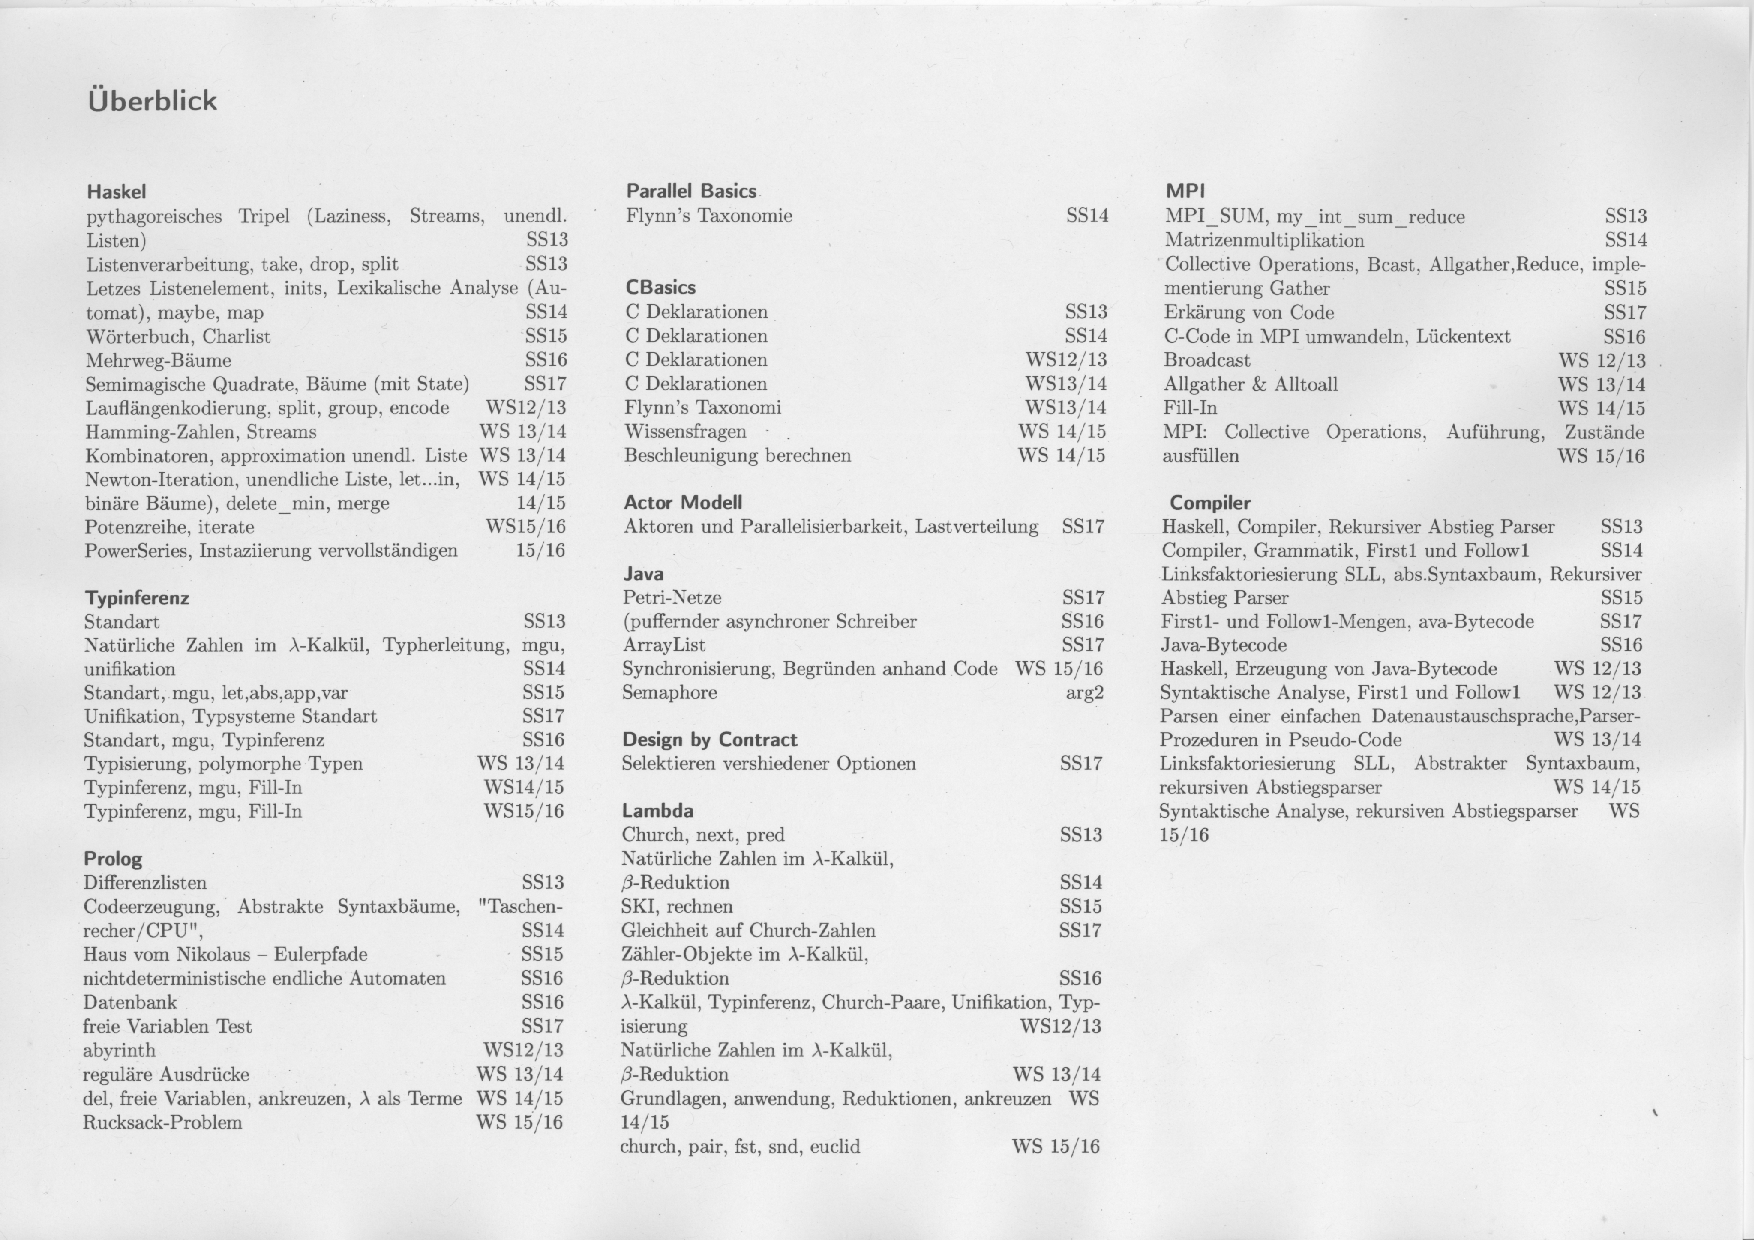
\includegraphics{imgs/TaskOverview.png}}
\end{sidewaysfigure}
\chapter{Fragen}
\section{Klausurrelevant}
\begin{itemize}
	\item X10 klausurrelevant?
\end{itemize}

\section{Design by Contract}
\subsection{JML}
\begin{itemize}
	\item Objekte non-Null Default: \href{http://www.eecs.ucf.edu/~leavens/JML/jmlrefman/jmlrefman_2.html#SEC16}{Reference}
	\item muss die Precondition Availability rule \slide{60}{25} erfüllt / eingehalten werden? Oder nur Best Practice?
\end{itemize}

\section{Compiler}
\subsection{First und Follow Mengen}
\begin{itemize}
	\item $Follow_k(x)$ auch wie folgt definierbar?:
		\begin{align*}
			Follow_k(x) &= \{ \cup\; First_k(y) | \exists m,y \in (V \cup \Sigma)^* : S \Rightarrow^* mxy \}\\
						&= \{ u \in \Sigma^k | \exists m,y \in (V \cup \Sigma)^*: \bigg(S \Rightarrow^* mxy\bigg) \wedge \bigg( u \in First_k(y) \bigg) \} \text{ (große Klammern hinzugefügt)}\\
						&= \{ u \in \Sigma^k | \exists m,y \in (V \cup \Sigma)^*: S \Rightarrow^* mxy \wedge u \in First_k(y) \} \text{ \slide{71}{379}}
		\end{align*}
	\item wie ist $Follow_k(x)$ definiert, wenn 
		$$S \nRightarrow mxy$$
		d.h. wenn \enquote{x} nie von S aus abgebildet wird? (bspw. $Follow_k(S)$, d.h. S ist nur Startzustand, wird aber durch keine Produktion / Abbildung erreicht?)\\
		\textbf{Annahme:} $Follow_k(x) = \{ \# \}$
	\item gilt $\# \in Follow_k(S)$ immer?
\end{itemize}
\subsection{Java-Bytecode}
\begin{itemize}
	\item was passiert wenn Typ der Stackvariablen nicht mit dem erwarteten Operationstyp übereinstimmt?\\
		z.B: oberste Variable auf Stack ist \enquote{3.5} (Double) und istore\_3 wird ausgeführt\\
		$\Rightarrow$ Exception?
	\item Unterschied zwischen \enquote{bipush} und \enquote{ldc} Befehlen
	\item wann \enquote{ldc} Befehl verwenden? \slide{73}{436}
\end{itemize} 

\chapter{Haskell}
\begin{itemize}
	\item equal:: \enquote{==}
	\item not equal:: \enquote{/=}
\end{itemize}

\funcSignature{changeListAt::(a -> a) -> Int -> [a] -> [a]} 
\exRef{SS 16, Nr. 1}\\
\texttt{changeListAt f i list}: Wendet auf das i-te Element (1. Element hat Index 0) der Liste \enquote{list} die Funktion f an.
\begin{lstlisting}
changeListAt f i []=[]
changeListAt f 0 (x:xs) = ((f x):xs)
changeListAt f i (x:xs) = x.(changeListAt f (i-1) xs)
\end{lstlisting}

\funcSignature{isPalindrom::Eq a => [a] -> Bool}
\texttt{isPalindrom list} überprüft es sich bei der Liste \enquote{list} um ein Palindrom handelt 
\begin{lstlisting}
isPalindrom xs = foldl (&&) True (zipWith (\x y -> x==y) xs (myRev1 xs))
\end{lstlisting}

\funcSignature{flatten::[[a]] -> [a]}
Transform a list, possibly holding lists as elements into a `flat' list by replacing each list with its elements (recursively). 
\begin{lstlisting}
data NestedList a = Elem a | List [NestedList a]

flatten (Elem a)      = [a]
flatten (List [])     = []
flatten (List (x:xs)) = (flatten x) ++ (flatten (List xs))
flatten (List [])     = []
\end{lstlisting}

\funcSignature{compress::Eq a => [a] -> [a]}
Entferne aufeinanderfolgende Duplikate in einer Liste
\begin{lstlisting}
compress []     = []
compress (x:xs) = x : (compress $ dropWhile (== x) xs)
\end{lstlisting}

\funcSignature{pack::Eq a => [a] -> [[a]]}
Speichere aufeinanderfolgende Duplikate aus der Eingabeliste in Unterlisten. Falls sich Elemente aus der Eingabeliste wiederholen und nicht direkt aufeinanderfolgen, werden diese in separate Unterlisten gespeichert.
\begin{lstlisting}
pack::Eq a => [a] -> [[a]]
pack [] = []
pack (x:xs) = (x:(filter (==x) xs)):(pack $ filter (/=x) xs)
\end{lstlisting}

\funcSignature{duplicate::[a] -> [a]}
Dupliziere die Elemente einer Liste
\begin{lstlisting}
duplicate []     = []
duplicate (x:xs) = x x:(duplicate xs)
\end{lstlisting}

\funcSignature{replicate::[a] -> Int -> [a]}
\texttt{replicate list n} repliziert die Elemente der Liste \enquote{list} n-mal
\begin{lstlisting}
repli xs n = concat [f x | x <- xs]
  where f x = take n (repeat x)
\end{lstlisting}

\funcSignature{dropEvery::[a] -> Int -> [a]}
\texttt{dropEvery list n} entfernt jedes n-te Element aus der Liste
$$\text{dropEvery [1,2,3,4] 2 == [1,3]}$$
\begin{lstlisting}
dropEvery list count = helper list count count
  where 
    helper [] _ _ = []
    helper (x:xs) count 1 = helper xs count count
    helper (x:xs) count n = x : (helper xs count (n - 1))
\end{lstlisting}

\funcSignature{rotate::[a] -> Int -> [a]}
\texttt{rotate list n} verschiebe die Elemente der Liste um n Stellen nach links
$$\text{rotate \enquote{abcdefgh} 3 == \enquote{defghabc}}$$
$$\text{rotate \enquote{abcdefgh} (-2) == \enquote{ghabcdef}}$$
\begin{lstlisting}
rotate xs n = drop nn xs ++ take nn xs
  where nn = n `mod` length xs
\end{lstlisting}
%\chapter{Haskell}
\begin{itemize}
	\item equal:: \enquote{==}
	\item not equal:: \enquote{/=}
\end{itemize}

\funcSignature{changeListAt::(a -> a) -> Int -> [a] -> [a]} 
\exRef{SS 16, Nr. 1}\\
\texttt{changeListAt f i list}: Wendet auf das i-te Element (1. Element hat Index 0) der Liste \enquote{list} die Funktion f an.
\begin{lstlisting}
changeListAt f i []=[]
changeListAt f 0 (x:xs) = ((f x):xs)
changeListAt f i (x:xs) = x.(changeListAt f (i-1) xs)
\end{lstlisting}

\funcSignature{isPalindrom::Eq a => [a] -> Bool}
\texttt{isPalindrom list} überprüft es sich bei der Liste \enquote{list} um ein Palindrom handelt 
\begin{lstlisting}
isPalindrom xs = foldl (&&) True (zipWith (\x y -> x==y) xs (myRev1 xs))
\end{lstlisting}

\funcSignature{flatten::[[a]] -> [a]}
Transform a list, possibly holding lists as elements into a `flat' list by replacing each list with its elements (recursively). 
\begin{lstlisting}
data NestedList a = Elem a | List [NestedList a]

flatten (Elem a)      = [a]
flatten (List [])     = []
flatten (List (x:xs)) = (flatten x) ++ (flatten (List xs))
flatten (List [])     = []
\end{lstlisting}

\funcSignature{compress::Eq a => [a] -> [a]}
Entferne aufeinanderfolgende Duplikate in einer Liste
\begin{lstlisting}
compress []     = []
compress (x:xs) = x : (compress $ dropWhile (== x) xs)
\end{lstlisting}

\funcSignature{pack::Eq a => [a] -> [[a]]}
Speichere aufeinanderfolgende Duplikate aus der Eingabeliste in Unterlisten. Falls sich Elemente aus der Eingabeliste wiederholen und nicht direkt aufeinanderfolgen, werden diese in separate Unterlisten gespeichert.
\begin{lstlisting}
pack::Eq a => [a] -> [[a]]
pack [] = []
pack (x:xs) = (x:(filter (==x) xs)):(pack $ filter (/=x) xs)
\end{lstlisting}

\funcSignature{duplicate::[a] -> [a]}
Dupliziere die Elemente einer Liste
\begin{lstlisting}
duplicate []     = []
duplicate (x:xs) = x x:(duplicate xs)
\end{lstlisting}

\funcSignature{replicate::[a] -> Int -> [a]}
\texttt{replicate list n} repliziert die Elemente der Liste \enquote{list} n-mal
\begin{lstlisting}
repli xs n = concat [f x | x <- xs]
  where f x = take n (repeat x)
\end{lstlisting}

\funcSignature{dropEvery::[a] -> Int -> [a]}
\texttt{dropEvery list n} entfernt jedes n-te Element aus der Liste
$$\text{dropEvery [1,2,3,4] 2 == [1,3]}$$
\begin{lstlisting}
dropEvery list count = helper list count count
  where 
    helper [] _ _ = []
    helper (x:xs) count 1 = helper xs count count
    helper (x:xs) count n = x : (helper xs count (n - 1))
\end{lstlisting}

\funcSignature{rotate::[a] -> Int -> [a]}
\texttt{rotate list n} verschiebe die Elemente der Liste um n Stellen nach links
$$\text{rotate \enquote{abcdefgh} 3 == \enquote{defghabc}}$$
$$\text{rotate \enquote{abcdefgh} (-2) == \enquote{ghabcdef}}$$
\begin{lstlisting}
rotate xs n = drop nn xs ++ take nn xs
  where nn = n `mod` length xs
\end{lstlisting}
\chapter{Theoretische Grundlagen}
\section{Äquivalenz}
\subsection{$\alpha$-Äquivalenz \slide{20}{166}}
gleicher Ausdruck / Funktion, nur andere Namen $\Rightarrow$ durch Umbenennung Transformation von $t_1$ zu $t_2$ möglich

\subsection{$\eta$-Äquivalenz \slide{20}{167}}
Zwei Funktionen sind gleich, falls Ergebnis gleich für alle Argumente

\subsection{Divergenz \slide{20}{182}}
Terme, die nicht zu einer Normalform auswerten, divergieren. Diese modellieren unendliche Ausführungen.

\subsection{Rekursionsoperator \slide{20}{184}}
$$Y= \lambda f.\; (\lambda x.\; f\; (x\; x))\; (\lambda x.\; f\; (x\; x))$$
mit 
$$f\; (Y\; f) \overset{\beta}{=} Y\; f$$ 
\todo[inline]{$\overset{\beta}{=}$ Bedeutung: Gleich nach vollständiger $\beta$-Reduktion?}

\subsection{Auswertungsstrategien}
\begin{compactitem}
	\item Volle $\beta$-Reduktion \slide{20}{177}: Jeder Redex kann jederzeit reduziert werden
	\item Normalenreihenfolge \slide{20}{177}: Immer der linkeste äußerste Redex (der Parameter zur Verfügung hat) wird reduziert
	\item Call-By-Name \slide{20}{189}: Reduziere linkesten äußersten Redex, der nicht von einem $\lambda$ umgeben ist\\
	$\Rightarrow$ Reduziere Argumente erst, wenn benötigt
	\item Call-By-Value \slide{20}{190}: Reduziere linkesten äußersten Redex, der nicht von einem $\lambda$ umgeben ist und dessen Argument ein Wert (d.h. max. ausgewertet, darf auch ein Lambda-Ausdruck sein) ist\\
	$\Rightarrow$ werte Argumente vor Funktionsaufruf aus, dann setze max. ausgewertete Argumente ein
\end{compactitem}

\subsection{Church-Zahlen \slide{20}{179ff}}
\begin{compactitem}
	\item Zahlen:
		\begin{align*}
			c_0 &= \lambda s.\; \lambda z.\; z\\
			c_1 &= \lambda s.\; \lambda z.\; s\; z\\
			c_2 &= \lambda s.\; \lambda z.\; s\; (s\; z)\\
				& \vdots \\
			c_n &= \lambda s.\; \lambda z.\; s^n\; z
		\end{align*}
	\item Operationen
		\begin{compactitem}
			\item Nachfolgerfunktion $succ = \lambda n.\; \lambda s.\; \lambda z.\; s\; (n\; s\; z)$
			\item Addition $plus = \lambda m.\; \lambda n.\; \lambda s.\; \lambda z.\; m\; s\; (n\; s\; z)$
			\item Multiplikation $times = \lambda m.\; \lambda n.\; \lambda s.\; n\; (m\; s) \overset{\eta}{=} \lambda m.\; \lambda n.\; \lambda s.\; \lambda z.\; n\; (m\; s)\; z$
			\item Potenzieren $exp = \lambda m.\; \lambda n.\; n\; m \overset{\eta}{=} \lambda m.\; \lambda n.\; \lambda s. \; \lambda z.\; n\; m\; s\; z$
			\item Subtraktion $sub = \lambda m.\; \lambda n.\; n\; pred\; m$\exRef{ÜB 5, Nr. 4}
				\begin{compactitem}
					\item $pair = \lambda a.\; \lambda b.\; \lambda f.\; f\; a\; b$
					\item $fst = \lambda p.\; p (\lambda a.\; \lambda b.\; a)$
					\item $snd = \lambda p.\; p (\lambda a.\; \lambda b.\; b)$
					\item $next = \lambda p.\; pair\; (snd\; p)\; (succ\; (snd\; p))$
					\item $pred = \lambda n.\; fst\; (n\; next\; (pair\; c_0\; c_0))$
				\end{compactitem}
			\item Vegleichsoperation \enquote{lessEq $m \leq n$} $lessEq = \lambda m.\; \lambda n.\; isZero\; (sub\; m\; n)$\exRef{ÜB 6, Nr. 2}
			\item Vegleichsoperation \enquote{greaterEq $m \geq n$} $greaterEq = \lambda m.\; \lambda n.\; isZero\; (sub\; n\; m)$
			\item Vergleichsoperation \enquote{eq $m == n$} $eq = \lambda m.\; \lambda n.\; (\lambda a.\; a)\; (lessEq\; m\; n)\; (greaterEq\; m\; n)\; c_{false}$
			\item $isZero = \lambda n.\; n\; (\lambda p.\; c_{false})\; c_{true}$\exRef{SS 14}
		\end{compactitem}
	\item boolsche Werte
		\begin{compactitem}
			\item True $c_{true} = \lambda t.\; \lambda f.\; t$
			\item False $c_{false} = \lambda t.\; \lambda f.\; f$
		\end{compactitem}
\end{compactitem}

\subsection{Rekursionsoperator Y \slide{20}{184}}
$$Y=\lambda f. (\lambda x. f (x\; x))(\lambda x.f(x\; x))$$
\begin{compactitem}
	\item Rekursionsoperator Y ist nicht typisierbar \slide{21}{205}
\end{compactitem}

\section{Typinferenz}
Bei Let-Polymorphismus angepasste Regeln von VAR und ABS \slide{22}{211}\\
\iffalse
\noindent\makebox[\textwidth]{
\begin{tabular}{|c|c|c|}
	\hline 
	Regel & Constraint & Bsp. \\ 
	\hline 
	CONST\begin{LARGE}$\frac{c\;\in\; Const}{\Gamma\; \vdash\; c\; :\; \tau_c}$\end{LARGE}
	& \multlineTable{CONST\begin{LARGE}$\frac{c\;\in\; Const}{\Gamma\; \vdash\; c\; :\; \alpha_1}:$\end{LARGE}\\ $\alpha_1 = Typ(c)$ }
	& \multlineTable{CONST\begin{LARGE}$\frac{1\;\in\; Const}{\Gamma\; \vdash\; 1\; :\; \alpha_1}:$\end{LARGE}\\ $\alpha_1 = Typ(1)=Int$ } 
	\\[5ex]
	\hline 
	VAR\begin{LARGE}$\frac{\Gamma(x)\;=\;\tau}{\Gamma\; \vdash\; x\; :\; \tau}$\end{LARGE} 
	& \multlineTable{VAR\begin{LARGE}$\frac{(x:\;\alpha_1)(x)\;=\;\alpha_2}{(x\;:\;\alpha_1)\; \vdash\; x\;:\; \alpha_2}:$\end{LARGE}\\ $\alpha_1 = \alpha_2$ }
	& \\[5ex]
	\hline 
	ABS\begin{LARGE}$\frac{\Gamma,\;x\;:\;\tau_1\; \vdash\; t\;:\;\tau_2}{\Gamma\; \vdash\; \lambda x.t:\; \tau_1\; \rightarrow\; \tau_2}$\end{LARGE}
	& \multlineTable{ABS\begin{LARGE}$\frac{\Gamma,\;x\;:\;\alpha_2\; \vdash\; t\;:\;\alpha_3}{\Gamma\; \vdash\; \lambda x.t\;:\; \alpha_1}:$\end{LARGE}\\ $\alpha_1 = \alpha_2\; \rightarrow\; \alpha_3$ }  
	&  \\[5ex]
	\hline 
	APP\begin{LARGE}$\frac{\Gamma\; \vdash\; t_1\;:\;\tau_2\; \rightarrow\; \tau \qquad \Gamma\; \vdash\; t_2\; :\; \tau_2}{\Gamma\; \vdash\; t_1\; t_2:\; \tau}$\end{LARGE}
	& \multlineTable{APP\begin{LARGE}$\frac{\Gamma\; \vdash\; t_1\;:\;\alpha_2\; \qquad \Gamma\; \vdash\; t_2\; :\; \alpha_3}{\Gamma\; \vdash\; t_1\; t_2\;:\; \alpha_1}:$\end{LARGE} \\ $\alpha_2 = \alpha_3 \rightarrow \alpha_1$ }  
	& \\[5ex]
	\hline
	LET\begin{LARGE}$\frac{\Gamma\; \vdash\; t_1\;:\;\tau_1 \quad \Gamma,\; x\;:\; ta(\tau_1,\;\Gamma)\;\vdash\; t_2\; :\; \tau_2}{\Gamma\; \vdash\; let\; x = t_1\; in\; t_2\; :\; \tau_2}$\end{LARGE}
	& \multlineTable{LET\begin{LARGE}$\frac{\Gamma\; \vdash\; t_1\;:\;\alpha_2 \quad \Gamma,\; x\;:\; ta(\alpha_2,\;\Gamma)\;\vdash\; t_2\; :\; \alpha_3}{\Gamma\; \vdash\; let\; x = t_1\; in\; t_2\; :\; \alpha_1}:$\end{LARGE} \\ $\alpha_2 = \alpha_3$}  
	& \\[5ex]
	\hline
\end{tabular} 
}
\fi 

\noindent\makebox[\textwidth]{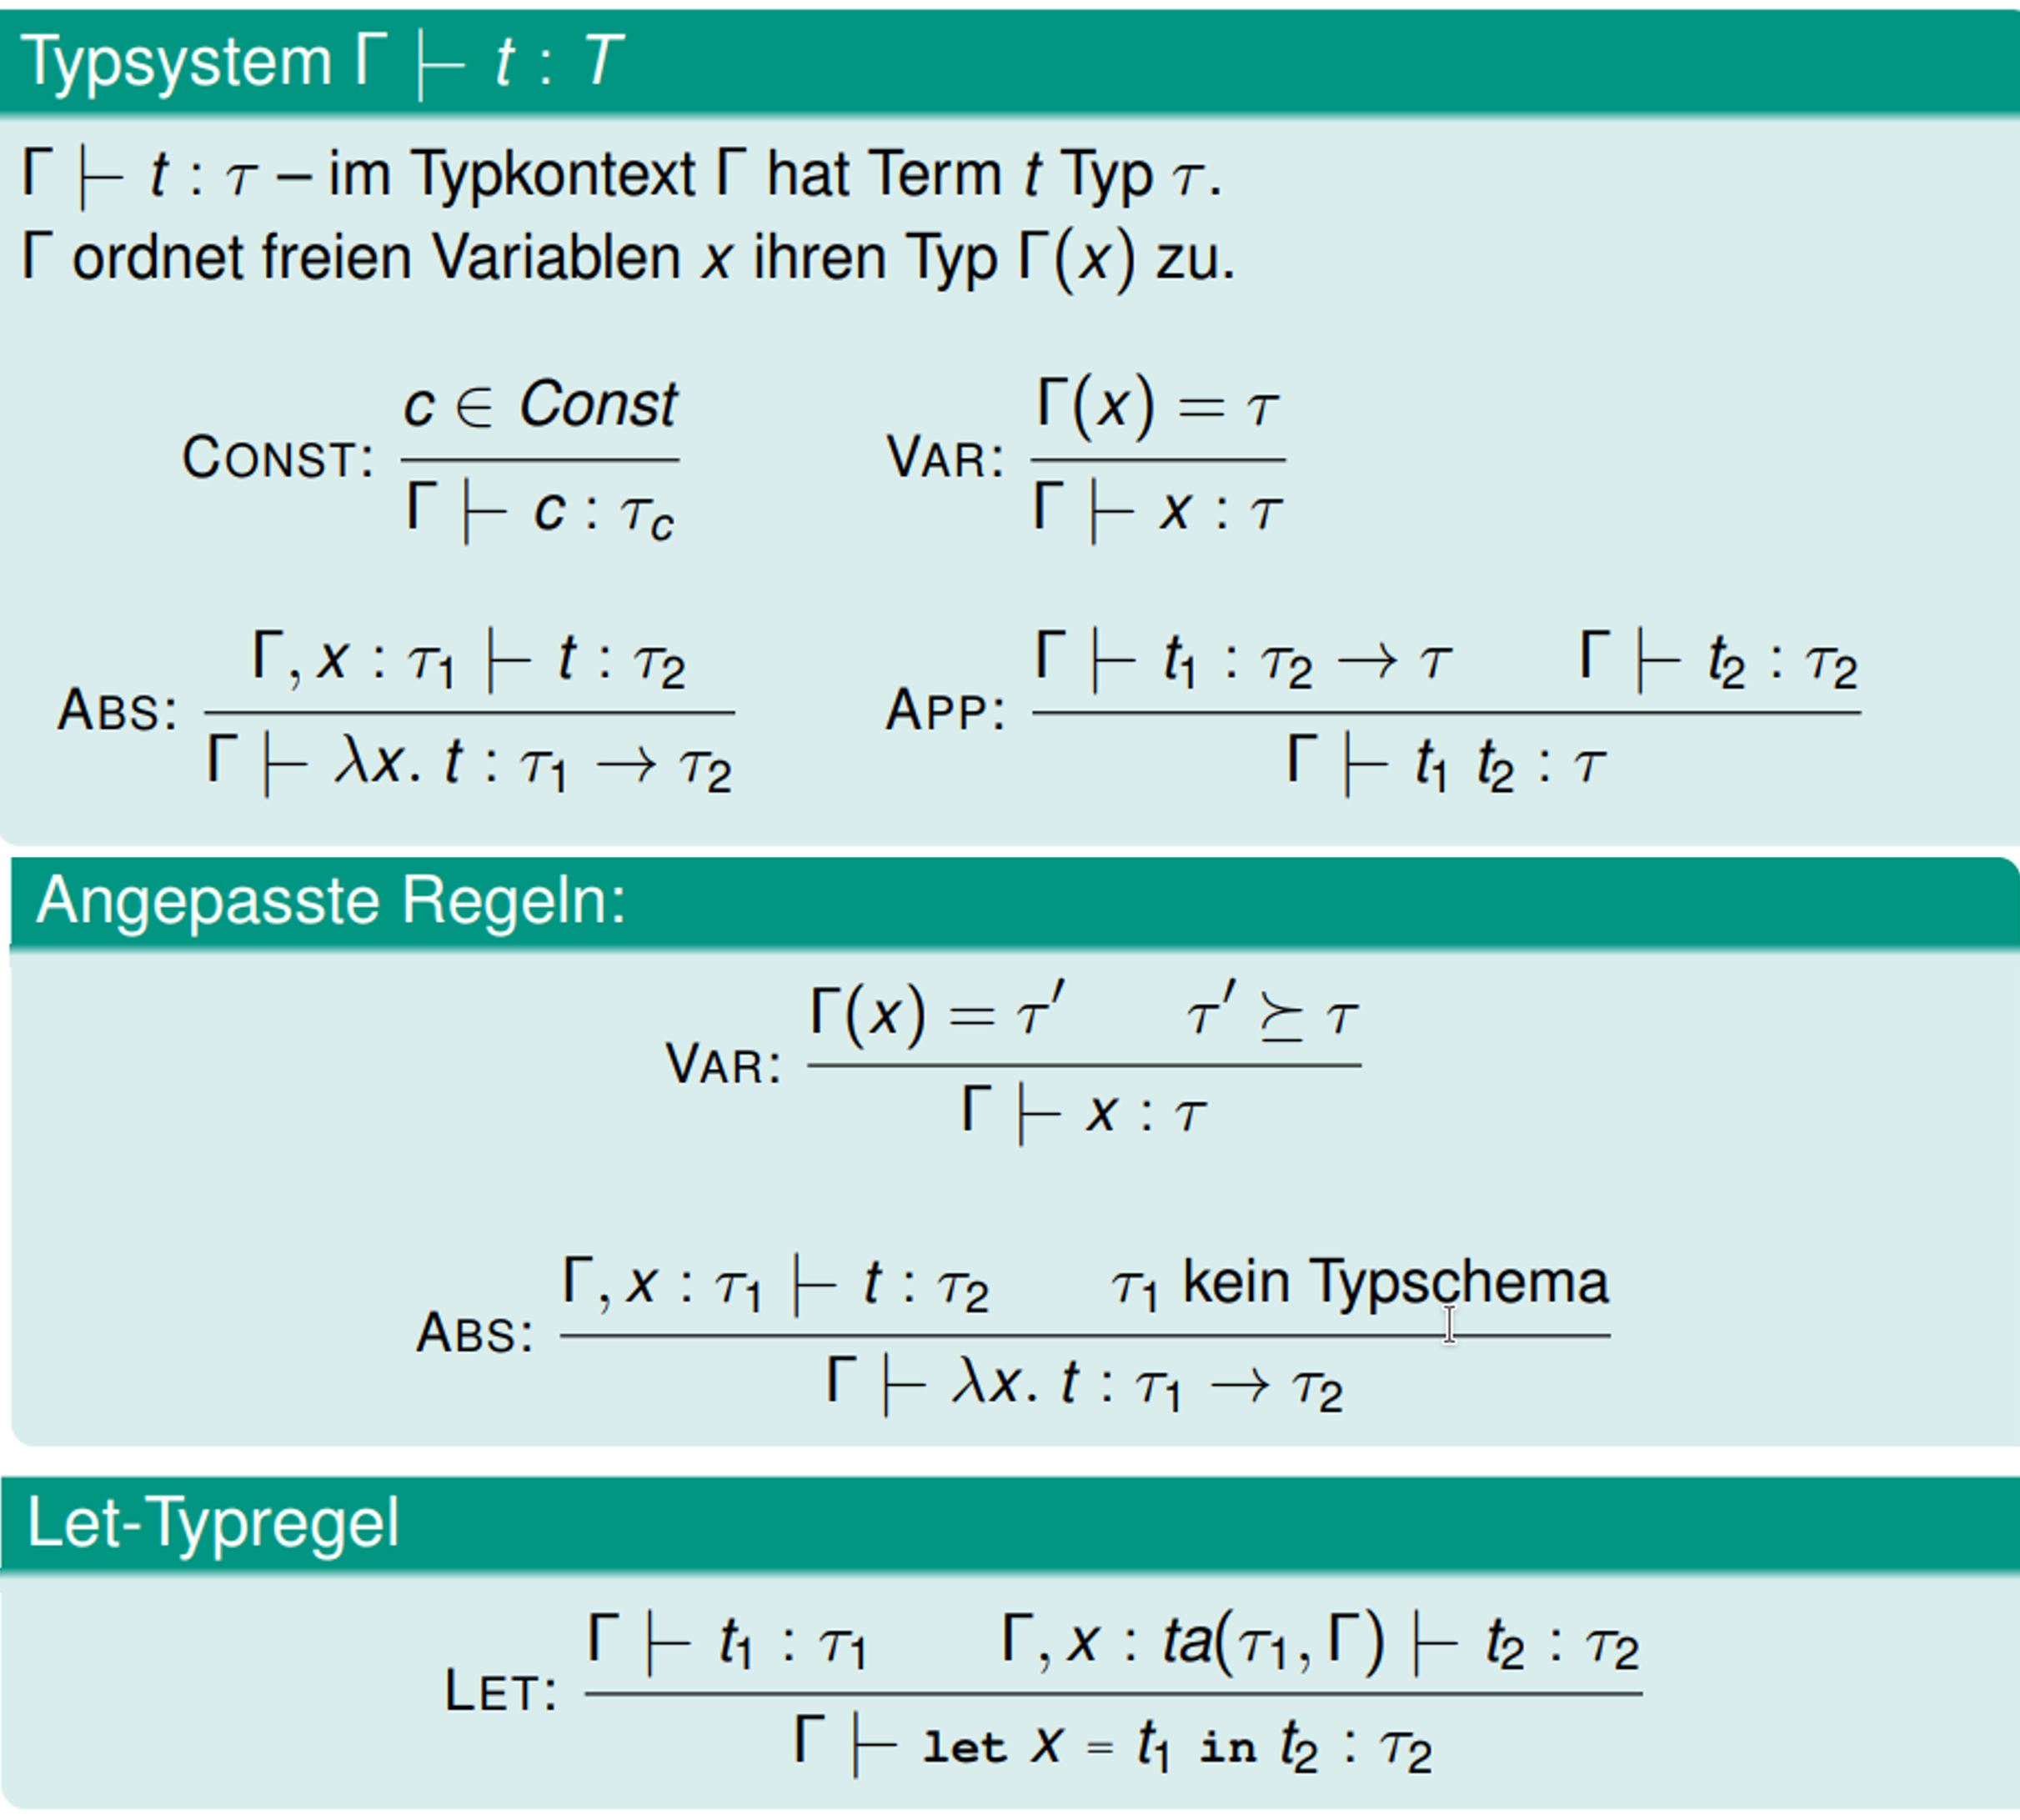
\includegraphics[scale=0.20]{imgs/TypinferenzCaptureCut.png}}

\lstset{language=Prolog} 
\chapter{Prolog}
\section{Vergleich arithmetischer Ausdrücke}
\begin{compactitem}
	\item gleich: \enquote{=:=}
	\item ungleich: \enquote{=\textbackslash =}
	\item kleiner: \enquote{$<$}
	\item kleiner-gleich : \enquote{$=<$}
	\item größer: \enquote{$>$}
	\item größer-gleich: \enquote{$>=$}
\end{compactitem}

\section{Funktionen für Listen}
\begin{compactitem}
	\item member \slide{31}{243}: Überprüfe ob Element in Liste enthalten
		\begin{lstlisting}
		member(X, [X|T]).
		member(X, [Y|T]):- member(X, T).
		\end{lstlisting}
	\item append \slide{31}{243}: Hänge eine Liste an eine andere
		\begin{lstlisting}
		append([],L, L).
		append([X|R], L, [X|T]):- append(R, L, T).
		\end{lstlisting}
		\enquote{Die Konkatenation von [] und L ist L. Wenn die Konkatenation von R und L die Liste T ergibt, dann ergibt die Konkatenation von [X|R] und L die Liste [X|T].}
	\item reverse \slide{31}{245}: 		
		\begin{lstlisting}
		reverse([],[]).
		reverse([X|R], Y):- reverse(R, Y1), append(Y1, [X], Y).
		\end{lstlisting}
		effizienter:
		\begin{lstlisting}
		reverse(X,Y):- reverse(X, [], Y).
		reverse([], Y, Y).
		reverse([X|R], A, Y):- reverse(R, [X|A], Y).
		\end{lstlisting}
	\item Quicksort \slide{31}{247}:
		\begin{lstlisting}
		qsort([],[]).
		qsort([X|R],Y):- split(X,R,R1,R2),
				 qsort(R1,Y1),
				 qsort(R2,Y2),
				 append(Y1,[X|Y2],Y).
		split(X,[],[],[]).
		split(X,[H|T],[H|R],Y):- X>H, split(X,T,R,Y).
		split(X,[H|T],R,[H|Y]):- X=<H, split(X,T,R,Y).
		\end{lstlisting}
	\item Listenpermutation \slide{31}{248}:
		\begin{lstlisting}
		permute([],[]).
		permute([X|R],P):- permute(R,P1),append(A,B,P1),append(A,[X|B],P).
		\end{lstlisting}
	\item lösche alle Elemente X aus Liste \exRef{Üb 8, Nr. 3}:
		\begin{lstlisting}
		del([],_,[]).
		del([X|T1],X,L2)    :- del(T1,X,L2).
		del([Y|T1],X,[Y|T2]):- del(T1,X,T2), not(X=Y).
		\end{lstlisting}	
	\item Listenlänge \exRef{WS 12/13, Nr. 3a}
		\begin{lstlisting}
		length([],0).
		length([_|R], NewLength):- length(R,Length), NewLength is Length +1.
		\end{lstlisting}
	\item Test auf Duplikate:
		\begin{lstlisting}
		noDuplicates([]).
		noDuplicates([H|T]):- not(member(H,T)), noDuplicates(T).
		\end{lstlisting}
	\item Entferne aufeinanderfolgende Duplikate:
		\begin{lstlisting}
		removeDuplicates([],[]).
		removeDuplicates([H|[H|T]], L):- removeDuplicates([H|T],L).
		removeDuplicates([H|T], [H|L]):- removeDuplicates(T,L).
		\end{lstlisting}
	\item Entferne alle Duplikate (auch wenn doppelte Elemente nicht direkt hintereinander sind):
		\begin{lstlisting}
		removeAllDuplicates([],[]).
		removeDuplicates([H|T], [H|L]):- deleteElem(T,H,L1), removeDuplicates(L1,L).
		\end{lstlisting}
\end{compactitem}

\chapter{Parallelprogrammierung}
\section{Grundlagen}
\subsection{Coffman-Bedingungen (Deadlock-Bedingungen) \slide{54}{47}}
Wenn alle vier der folgenden Bedingungen zutreffen, liegt ein Deadlock vor.
Deadlocks können verhindert werden, indem immer mindestens eine Bedingung nicht erfüllt ist, d.h. nicht alle auf einmal erfüllt sein können.
\begin{compactenum}
	\item \textbf{Mutual exclusion}
		\begin{compactitem}
			\item beschränkter Zugriff auf eine Ressource
			\item Ressource kann nur mit einer beschränkten Anzahl von Nutzern geteilt werden
		\end{compactitem}
	\item \textbf{Hold and wait}: Warten auf alle benötigten Ressourcen, während die Kontrolle über bisher zugesprochene (mind. eine) Ressourcen behalten wird.
	\item \textbf{No preemption}: Zugewiesene Ressourcen können nur freiwillig zurückgegeben werden, die Rückgabe kann nicht erzwungen werden.
	\item \textbf{Circular Wait: }Möglichkeit von Kreisen in Ressourcen-Anfragen Graph:\\
				Zyklische Kette von Prozessen, die bereits Ressourcen (mind. eine) erhalten haben und gleichzeiig auf weitere Ressourcen warten, welche jeweils dem nächsten Prozess in der zirkulären Kette zugesprochen wurden.
\end{compactenum}

\subsection{Flynn's Taxonomy \slide{51}{13}\exRef{Grafiken von SS 14, Nr. 6}}
\todo[inline]{Grafiken korrekt? Vgl. SIMD und MISD}
\noindent\makebox[\textwidth]{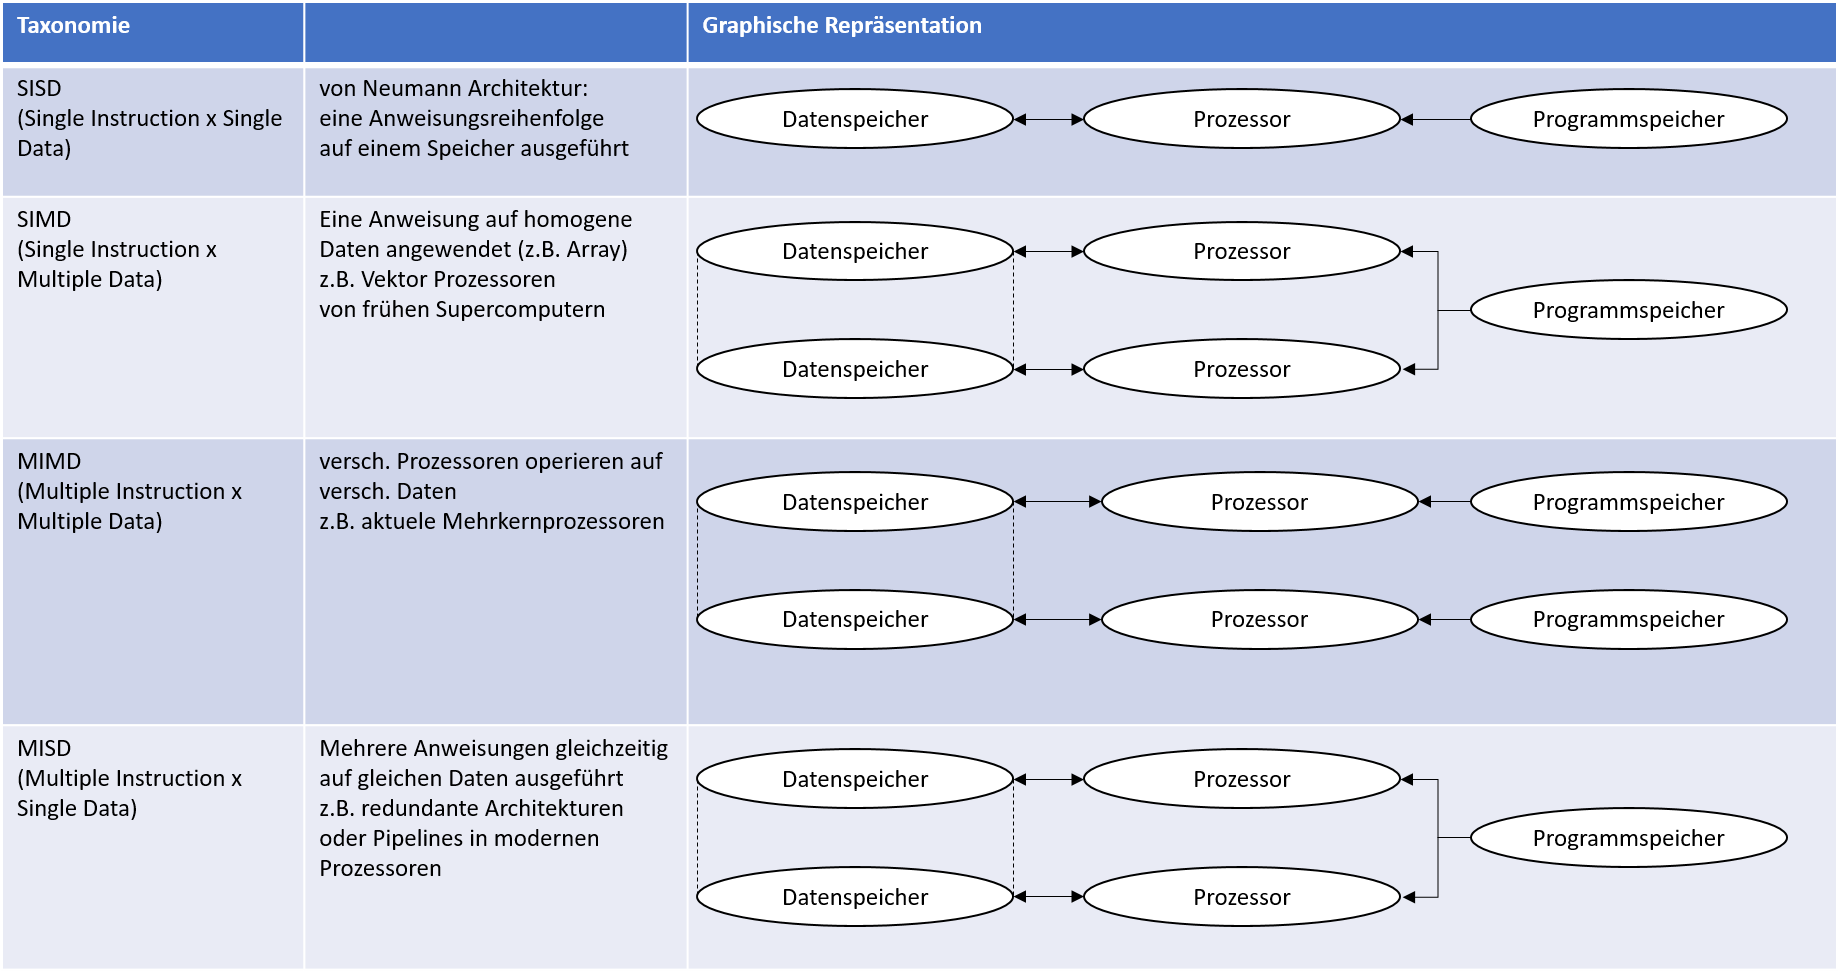
\includegraphics[width=200mm]{imgs/FlynnsTaxonomy.png}}

\subsection{Beschleunigung: Amdahl's Law \slide{51}{17}}
\myparagraph{Beschleunigung eines Algo durch die Verwendung von n Prozessoren:}
$$S(n) = \frac{T(1)}{T(n)}=\frac{\text{Ausführungszeit mit einem Prozessor}}{\text{Ausführungszeit mit n Prozessoren}}$$
\myparagraph{maximale Beschleunigung durch parallele Ausführung mit n Prozessoren:}
$$S(n)= \frac{1}{(1-p)+ \frac{p}{n}}$$
p: parallelisierbarer prozentualer Anteil des Programms

\section{MPI}
\begin{compactitem}
	\item \texttt{MPI\_Comm\_WORLD}: Standard Communicator	
	\item \texttt{MPI\_Init(\&argc, \&args)}: initialisiere MPI
	\item \texttt{MPI\_Finalize()}: Clean-Up nach Ausführung von MPI
	\item \texttt{MPI\_Comm\_rank(MPI\_Comm\_WORLD, \&my\_rank)}: my\_rank enthält den Rank des aktuellen Prozesses
	\item \texttt{MPI\_Comm\_size(MPI\_Comm\_WORLD, \&size)}: size enthält Gesamtanzahl von Prozessen
	\item \texttt{MPI\_Barrier(MPI\_Comm\_WORLD)}: Barriere, blockiert bis alle Prozesse die Barriere aufgerufen haben
	\item \texttt{MPI\_Send(void* buffer, int count, MPI\_Datatype datatype, int dest, int tag, MPI\_Comm comm)}
	\item \texttt{MPI\_Recv(void* buffer, int count, MPI\_Datatype datatype, int source, int tag, MPI\_Comm comm, MPI\_Status* status)}
\end{compactitem}

\section{Java}

\chapter{Design by Contract}
\section{JML}
\subsection{Basic Syntax}
\begin{table}[h]
	\centering
	\label{my-label}
	\begin{tabular}{l|l}
		Syntax    & Bedeutung      															\\ \hline
		$a ==> b$ & a impliziert b 															\\ \hline
		$a <==>$  & a und b äquivalent            											\\ \hline
		$a <=!=>$  & a und b \textbf{nicht} äquivalent ($a \nleftrightarrow b$)            	\\ \hline
		\textbackslash result  & Ergebnis der Methode            							\\ \hline
		\textbackslash old(E)  & Wert von E, bevor die Methode ausgeführt wurde        		\\ \hline	
		(\textbackslash forall declaration; range-expression; body-expression)  
		& \multlineTable{(\textbackslash forall int i; 0 \textless = i \&\& i \textless size; \textbackslash old(elements[i])==elements[i])\\ für alle i zwischen 0 und \enquote{size} gilt: \textbackslash old(elements[i])==elements[i])}\\ \hline	
		(\textbackslash exists declaration; range-expression; body-expression)  
		& \multlineTable{(\textbackslash exists int i; 0 \textless = i \&\& i \textless size; \textbackslash old(elements[i])==elements[i])\\ es gibt ein i zwischen 0 und \enquote{size}, für das gilt:\\ \textbackslash old(elements[i])==elements[i])}\\ \hline
	\end{tabular}
\end{table}
\chapter{Compiler}
\section{Java-Bytecode \href{https://docs.oracle.com/javase/specs/jvms/se10/jvms10.pdf}{The Java Virtual Machine Specification}}

Class-Datei disassemblen: \href{https://docs.oracle.com/javase/7/docs/technotes/tools/windows/javap.html}{javap}

\subsection{Präfixe / Suffixe}
\begin{table}[h]
	\centering
	\label{my-label}
	\begin{tabular}{l|l}
		Präfix / Suffix	& Operand Typ\\ \hline
		i	&	integer		\\ \hline
		l	&	long		\\ \hline
		s	&	short		\\ \hline
		b	&	byte		\\ \hline
		c	&	character	\\ \hline
		f	&	float		\\ \hline
		d	&	double		\\ \hline
		a	&	reference	\\
	\end{tabular}
\end{table}
\subsection{Lesen / Schreiben von lokalen Variablen}
\begin{table}[h]
	\centering
	\label{my-label}
	\begin{tabular}{l|l|l|l}
		Befehl & Parameter & Beschreibung & Beispiel \\ \hline
		iconst\_x	&	\multlineTable{$x\in \{0,1,2,3,4,5,m1\}$\\ } & \multlineTable{lädt die int-Konstante x\\ m1 steht für Konstante \enquote{-1}} & \multlineTable{\texttt{iconst\_1}\\ lädt den int-Wert \enquote{1} auf den Stack} \\ \hline
		\textbf{TYPE}load\_x	& 	\multlineTable{x: Index der lokalen\\ Variable $x\in \{ 0,1,2,3 \}$\\ (x gehört zum Befehl,\\ es gibt pro x ein Befehl;\\ d.h. x ist keine Variable) }	&	\multlineTable{lädt den Wert der Variable mit Typ\\ \enquote{TYPE} mit Index x auf den Stack} 	& \multlineTable{\texttt{iload\_2}\\ lade Wert von der Variable mit\\ Index 2 und dem Typ \enquote{Integer}}      \\ \hline
		
		\textbf{TYPE}store\_x	&	\multlineTable{x: Index der Variable\\ $x\in \{ 0,1,2,3 \}$\\ (x gehört zum Befehl,\\ es gibt pro x ein Befehl;\\ d.h. x ist keine Variable) }	&	\multlineTable{speichert den obersten Wert auf dem\\ Stack mit Typ \enquote{TYPE} in Variable\\ mit Index x}	& \multlineTable{\texttt{istore\_2}\\ speichere den obersten Wert auf\\ dem Stack vom Typ \enquote{Integer}\\ in Variable 2 }	\\ \hline
		
		\textbf{TYPE}load x	& \multlineTable{x: Index der lokalen\\ Variable $0 \leq x \leq 255$\\ (x mit 1 Byte darstellbar) }	&	\multlineTable{lädt den Wert der Variable mit Typ\\ \enquote{TYPE} mit Index x auf den Stack} 	& \multlineTable{\texttt{iload 7}\\ lade Wert von der Variable mit\\ Index 7 und dem Typ \enquote{Integer}}      \\ \hline
		
		\textbf{TYPE}store x	& \multlineTable{x: Index der lokalen\\ Variable $0 \leq x \leq 255$\\ (x mit 1 Byte darstellbar) }	&	\multlineTable{speichert den obersten Wert auf dem\\ Stack mit Typ \enquote{TYPE} in Variable\\ mit Index x}	& \multlineTable{\texttt{istore 7}\\ speichere den obersten Wert auf\\ dem Stack vom Typ \enquote{Integer}\\ in Variable 7}	\\ \hline	
		
		bipush const& \multlineTable{const: konstanter Wert,\\ der auf den Stack geladen\\ werden soll} & \multlineTable{Lade den geg. konstanten Wert\\ auf den Stack} & \multlineTable{bipush 10\\ Lade den Wert 10 auf den Stack} \\ \hline	
		
		ldc & \open  & Beschreibung & Beispiel \\ \hline
	\end{tabular}
\end{table}
\myparagraph{Vergleich \enquote{iload\_x} vs. \enquote{iload x}}
\begin{itemize}
	\item \enquote{iload\_x} (mit Unterstrich): $x \in \{ 0,1,2,3 \}$ ist ein (einziger) Befehl, ohne Parameter. \enquote{x} ist schon im Opcode enthalten. Der Befehl besteht aus 1 Byte.
	\item \enquote{iload x} (ohne Unterstrich): $0 \leq x \leq 255$ ist ein Befehl, mit Parameter \enquote{x}. x ist nicht im Opcode enthalten. \enquote{iload x} funktioniert mit allen Zahlen x, die in ein Byte passen.
\end{itemize}
Da die Befehle mit Unterstrich Platz sparen, werden sie von realen Compilern bevorzugt; vorausgesetzt x ist klein genug.

\subsection{Lesen / Schreiben von Feldern}
\begin{table}[h]
	\centering
	\label{my-label}
	\begin{tabular}{l|l|l|l}
		Befehl & Parameter & Beschreibung & Beispiel \\ \hline
		
		putfield & \open & Beschreibung & Beispiel \\ \hline	
		
		getfield & \open & Beschreibung & Beispiel \\ \hline		
		
	\end{tabular}
\end{table}

\subsection{Sprungbefehle}
\begin{table}[h]
	\centering
	\label{my-label}
	\begin{tabular}{l|l|l|l|}
		Befehl & Parameter  & Beschreibung & Beispiel \\ \hline		
		ifle LABEL & \multlineTable{LABEL: Label, zu dem\\ gesprungen werden soll,\\ falls die Bedingung erfüllt ist}   & \multlineTable{Wenn der oberste Wert auf dem\\ Stack \textbf{kleiner oder gleich 0} ist,\\ dann springe zu dem geg. Label} & \multlineTable{ifle then\\ springe zu Label \enquote{then},\\ 
			\slide{73}{411} } \\ \hline		
			
		ifge LABEL & \multlineTable{LABEL: analog zu \enquote{ifle} }   & \multlineTable{Wenn der oberste Wert auf dem\\ Stack \textbf{größer oder gleich 0} ist,\\ dann springe zu dem geg. Label} & \multlineTable{ifge then\\ analog zu \enquote{ifle} } \\ \hline
		
		ifeq LABEL & \multlineTable{LABEL: analog zu \enquote{ifle}}   & \multlineTable{Wenn der oberste Wert\\ auf dem Stack \textbf{gleich 0} ist,\\ dann springe zu dem geg. Label} & \multlineTable{ifeq then\\  analog zu \enquote{ifle} } \\ \hline
		
		ifne LABEL & \multlineTable{LABEL: analog zu \enquote{ifle}}   & \multlineTable{Wenn der oberste Wert\\ auf dem Stack \textbf{nicht gleich 0} ist,\\ dann springe zu dem geg. Label} & \multlineTable{ifne then\\  analog zu \enquote{ifle} } \\ \hline	
		
		ifgt LABEL & \multlineTable{LABEL: analog zu \enquote{ifle}}   & \multlineTable{Wenn der oberste Wert\\ auf dem Stack \textbf{größer 0} ist,\\ dann springe zu dem geg. Label} & \multlineTable{ifgt then\\  analog zu \enquote{ifle} } \\ \hline		
		
		iflt LABEL & \multlineTable{LABEL: analog zu \enquote{ifle}}   & \multlineTable{Wenn der oberste Wert\\ auf dem Stack \textbf{kleiner 0} ist,\\ dann springe zu dem geg. Label} & \multlineTable{iflt then\\  analog zu \enquote{ifle} } \\ \hline \hline	
		
		ifnull LABEL & \multlineTable{LABEL: analog zu \enquote{ifle}}  & \multlineTable{Wenn der oberste Wert (/Referenz)\\ auf dem Stack \textbf{\texttt{NULL} ist},\\ dann springe zu dem geg. Label} & \multlineTable{ifnull then\\  analog zu \enquote{ifle}} \\ \hline	
			
		ifnonnull LABEL & \multlineTable{LABEL: analog zu \enquote{ifle}}  & \multlineTable{Wenn der oberste Wert (/Referenz)\\ auf dem Stack \textbf{nicht \texttt{NULL} ist},\\ dann springe zu dem geg. Label} & \multlineTable{ifnonnull then\\  analog zu \enquote{ifle} }\\ \hline \hline
		
		if\_icmpeq LABEL & \multlineTable{LABEL: analog zu \enquote{ifle}}  & \multlineTable{Wenn die beiden obersten Integer-\\Werte auf dem Stack \textbf{gleich} sind,\\ springe zu dem geg. Label} & \multlineTable{if\_icmpeq then\\ springe zu then\\ \slide{73}{429} } \\ \hline
		
		if\_icmpne LABEL & \multlineTable{LABEL: analog zu \enquote{ifle}}  & \multlineTable{Wenn die beiden obersten Integer-\\Werte auf dem Stack \textbf{nicht gleich}\\ sind, springe zu dem geg. Label} &  \multlineTable{if\_icmpne then\\ analog zu \enquote{if\_icmpeq} } \\ \hline
		
		if\_icmpge LABEL 
		& \multlineTable{LABEL: analog zu \enquote{ifle}}  
		& \multlineTable{Wenn der oberste Integer-Wert auf\\ dem Stack \textbf{gleich oder größer} als\\ der zweite ist, springe zu dem geg. Label} 
		&  \multlineTable{if\_icmpge then\\ analog zu \enquote{if\_icmpeq}} \\ \hline
		
		if\_icmpgt LABEL 
		& \multlineTable{LABEL: analog zu \enquote{ifle}}  
		& \multlineTable{Wenn der oberste Integer-Wert\\ auf dem Stack \textbf{größer} als der\\ zweite ist, springe zu dem geg. Label} 
		&  \multlineTable{if\_icmpgt then\\ analog zu \enquote{if\_icmpeq}} \\ \hline
		
		if\_icmple LABEL & \multlineTable{LABEL: analog zu \enquote{ifle}}  
		& \multlineTable{Wenn der oberste Integer-Wert auf\\ dem Stack \textbf{kleiner oder gleich} als\\ der zweite ist, springe zu dem geg. Label} 
		&  \multlineTable{if\_icmple then\\ analog zu \enquote{if\_icmpeq}} \\ \hline
		
		if\_icmplt LABEL & \multlineTable{LABEL: analog zu \enquote{ifle}}  & \multlineTable{Wenn der oberste Integer-Wert auf\\ dem Stack \textbf{kleiner} als der zweite ist,\\ springe zu dem geg. Label} &  \multlineTable{if\_icmplt then\\ analog zu \enquote{if\_icmpeq}} \\ \hline \hline
		
		goto LABEL	& \multlineTable{LABEL: analog zu \enquote{ifle}}  & \multlineTable{Springe bedingungslos zu dem geg.\\ Label} & \multlineTable{goto done\\ springe zu Label \enquote{done}\\ \slide{73}{411} }\\ \hline		
	\end{tabular}
\end{table}
\subsection{Methodenaufrufe}
\begin{table}[h]
	\centering
	\label{my-label}
	\caption{\href{https://www.javaworld.com/article/2860079/learn-java/dynamic-101.html}{Quelle}}
	\begin{tabular}{l|l|l|l|}
		Befehl & Parameter & Beschreibung & Beispiel \\ \hline
		
		invokevirtual \#INDEX 
		& \multlineTable{INDEX: Index der\\ aufzurufenden Methode} 
		& \multlineTable{Rufe die \textbf{nicht statische, public}\\ \textbf{oder protected} Methode mit dem\\ geg. Index auf. Die Parameter der\\ Methode werden automatisch in den\\ Operandenstack geladen, \textbf{beginnend}\\ \textbf{bei Variablen-Index 1}\\ (Variablen-Index 0: this-Variable / Referenz)} 
		& \multlineTable{invokevirtual \#2\\  Rufe die Methode\\ mit Index 2 auf\\ \slide{73}{419} } \\ \hline
		
		invokestatic \#INDEX 
		& \multlineTable{INDEX:  analog zu\\ \enquote{invokevirtual}} 
		& \multlineTable{Rufe die \textbf{statische} Methode mit dem\\ geg. Index auf. Die Parameter der\\ Methode werden automatisch in den\\ Operandenstack geladen, \textbf{beginnend}\\ \textbf{bei Variablen-Index 0}\\ (statische Methode, somit keine \enquote{this}-Variable)} 
		& \multlineTable{invokestatic \#2\\ analog zu \enquote{invokevirtual}}\\  \hline
		
		invokespecial \#INDEX 
		& \multlineTable{INDEX:  analog zu\\ \enquote{invokevirtual}} 
		& \multlineTable{Rufe die \textbf{private, Superklassen-}\\ \textbf{oder Konstruktor-} Methode\\ mit dem geg. Index auf. Die Parameter der\\ Methode werden automatisch in den\\ Operandenstack geladen, \textbf{beginnend}\\ \textbf{bei Variablen-Index 1}\\ (Variablen-Index 0: this-Variable / Referenz)} 
		& \multlineTable{invokespecial \#2 \\ analog zu \enquote{invokevirtual}} \\ \hline
		
		invokeinterface \#INDEX 
		& \multlineTable{INDEX:  analog zu\\ \enquote{invokevirtual}} 
		& \multlineTable{Rufe eine \textbf{Interface} Methode auf,\\ wobei Implementierung des\\ aufrufenden Objektes verwendet wird} 
		& \multlineTable{invokeinterface \#2 \\ analog zu \enquote{invokevirtual}} \\ \hline
		
		invokedynamic \#INDEX 
		& \multlineTable{INDEX:  analog zu\\ \enquote{invokevirtual}} 
		& \open 
		& \multlineTable{invokedynamic \#2 \\ analog zu \enquote{invokevirtual}} \\ \hline		
	\end{tabular}
\end{table}

\subsection{Objekterzeugung}
\begin{table}[h]
	\centering
	\label{my-label}
	\begin{tabular}{l|l|l|l}
		Befehl & Parameter & Beschreibung & Beispiel \\ \hline
		
		newarray TYPE& \multlineTable{TYPE: Typ der\\ Array-Werte} & \multlineTable{Erstelle ein Array mit Werten des geg. Typ\\ und der Größe des obersten Stack-Wertes.} & \multlineTable{newarray int\\ Erstelle ein int-Array} \\ \hline	
		
	\end{tabular}
\end{table}

\subsection{Arithmetische Berechnungen}
\begin{table}[h]
	\centering
	\label{my-label}
	\begin{tabular}{l|l|l|l}
		Befehl & Parameter & Beschreibung & Beispiel \\ \hline
		
		\textbf{TYPE}mul & - & \multlineTable{multipliziert zwei Werte vom Typ\\ \enquote{TYPE} und lädt das Ergebnis als\\ obersten Wert auf den Stack} & \multlineTable{\texttt{imul}} \\ \hline
		
		\textbf{TYPE}div & - & \multlineTable{dividiert zwei Werte vom Typ\\ \enquote{TYPE} und lädt das Ergebnis als\\ obersten Wert auf den Stack} & \multlineTable{\texttt{idiv}} \\ \hline
		
		\textbf{TYPE}add & - & \multlineTable{addiert zwei Werte vom Typ\\ \enquote{TYPE} und lädt das Ergebnis als\\ obersten Wert auf den Stack} & \multlineTable{\texttt{iadd}} \\ \hline
		
		\textbf{TYPE}sub & - & \multlineTable{subtrahiert zwei Werte vom Typ\\ \enquote{TYPE} und lädt das Ergebnis als\\ obersten Wert auf den Stack} & \multlineTable{\texttt{iadd}} \\ \hline
		
		\textbf{TYPE}neg & - & \multlineTable{negiert einen Wert vom Typ\\ \enquote{TYPE} und lädt das Ergebnis als\\ obersten Wert auf den Stack} & \multlineTable{\texttt{ineg}} \\ \hline		
		
		iinc index, const & \multlineTable{index:\\ Index der zu\\ inkrementierenden Variable\\ const:\\ Wert um den die Variable\\ inkrementiert werden soll}  & \multlineTable{Inkrementiere die Variable mit dem\\ geg. Index um den geg. konstanten\\ Wert} & \multlineTable{iinc 1, 1\\ inkrementiere die Variable\\ mit Index 1 um 1\\ iinc 1, -1\\ inkrementiere die Variable\\ mit Index 1 um (-1) } \\ \hline		
	\end{tabular}
\end{table}

\end{document}